\problemname{Pappershögen}
Idag ska Sven skulle göra i ordning sitt kontor när han stötte till sin hög med viktiga papper.
Helt plötsligt råkar Sven välta ner papperna på golvet och de hamner helt huller om buller. Det blir oordning- Katastof!
Sven samlar kvickt ihop papperna i en hög, men glömde att vissa av papperna hade hamnat upp och ner.
Sven gillar inte oordning och vill ha alla sina papper med rätt sida upp.
Hjälp Sven att hitta ett sätt att vända till rätta alla papper i högen.

Det visar sig dock att Sven är lite petig.
Efter att det just har blivit oordning känner Sven att ingenting får bli en röra igen.
Därför har Sven bestämt sig för att han *måste* behålla papprena i en hög.
Det enda han då kan göra är att ta de översta k papperna (han kan ta hela högen), vända bunten av dem uppockner och lägga tillbaka dem överst i högen.
Som den hårt arbetande isbjörn han är kan Sven tänka sig att göra uppemot $500\,000$ vändningar innan arbetsdagen är slut.

\begin{figure}[h]
	\centering
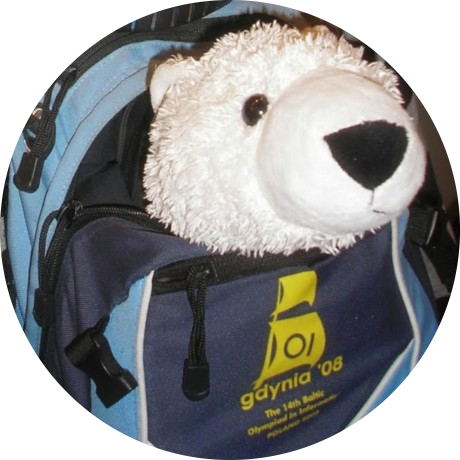
\includegraphics[width=0.5\textwidth]{sven-circular.png}
\caption{Sven}
\end{figure}

\section*{Indata}
Den första raden innehåller ett heltal: $1\leq N \leq 10^5$, antalet papper i högen.
Därefter följer $N$ tecken, där varje tecken antingen är ``U'' för att pappret är vänt rätt, eller ``N'' för att det är vänt fel. 

\section*{Utdata}
Skriv ut ett heltal $M$, ett antal vändningar som Sven kan göra för att få sin hög i ordning. För full poäng måste  $M \leq 500\,000$.
Skriv sedan ut $M$ heltal, antalet papper Sven ska vända för att rättvända alla papper. Varje tal måste vara minst $1$.

\section*{Poängsättning}
Din lösning kommer att testas på en mängd testfallsgrupper.
För att få poäng för en grupp så måste du klara alla testfall i gruppen.

\noindent
\begin{tabular}{| l | l | p{12cm} |}
  \hline
  Grupp & Poängvärde & Gränser \\ \hline
  $1$   & $10$       & $N=1$ \\ \hline
  $2$   & $20$       & $N \leq 10$ Sven behöver inte fler än $5$ vändningar. \\ \hline
  $3$   & $10$       & $N \leq 200$ det finns mest 2 felvända papper. \\ \hline
  $4$   & $10$       & Vart annat papper är felvänt. \\ \hline
  $5$   & $20$       & $N \leq 1000$ \\ \hline
  $6$   & $30$       & Inga ytterligare begränsningar  \\ \hline
\end{tabular}



\section*{Förklaring av exempelfall}
I första exemplet kan sven vända på 
I andra exemplet finns det $7$ lediga vägar. Denna uppfyller andra testgruppen.
